\documentclass{wissdoc}
%\documentclass[oneside]{wissdoc}
% ----------------------------------------------------------------
% Diplomarbeit - Hauptdokument
% ----------------------------------------------------------------
% wissdoc Optionen: draft, relaxed, pdf, oneside --> siehe wissdoc.cls
% ------------------------------------------------------------------
% Packages für Deckblatt
\usepackage[absolute]{textpos} 	%Textboxen an absolute Position setzen
\usepackage{setspace}						%Zeilenabstand anpassen
\usepackage{color}							%Farbige Schrift
\usepackage{graphicx}						%Einbinden von Grafiken

% Weitere packages: (Dokumentation dazu durch "latex <package>.dtx")
% \usepackage{varioref}
% \usepackage{verbatim}
% \usepackage{float}    %z.B. \floatstyle{ruled}\restylefloat{figure}
\usepackage{subfigure}
\usepackage[ngerman]{babel}
\usepackage[T1]{fontenc}
\usepackage[ansinew]{inputenc}

% Zeilenabstand nach Vorgabe - Falls gefordert
%\setstretch{1,3} 

% Inhaltsangabe auf Unterabschnitte(2 Ebenen) begrenzen
\setcounter{tocdepth}{2}


% \usepackage{color}    % Farbiger/grauer Text
% \usepackage{colortbl}   % Farbige/graue Tabellenzeilen und -spalten!! <--
% \usepackage{fancybox} % für schattierte,ovale Boxen etc.
% \usepackage{tabularx} % automatische Spaltenbreite
% \usepackage{supertab} % mehrseitige Tabellen
%% ---------------- end of usepackages -------------

%% Informationen für die PDF-Datei
\hypersetup{pdfauthor={Max Mustermann},%
            pdftitle={Bachelorarbeit},%
            pdfsubject={Titel der Arbeit},%
            pdfkeywords={Forschung, Entwicklung, Funktechnik},%
            pdfproducer={LaTeX},%
            pdfcreator={pdfLaTeX}
}

% Macros, nicht unbedingt notwendig
%%%%%%%%%%%%%%%%%%%%%%%%%%%%%%%%%%%%%%%%%%%%%%%%%%%%%%%%%%
% macros.tex -- einige mehr oder weniger nuetzliche Makros
%%%%%%%%%%%%%%%%%%%%%%%%%%%%%%%%%%%%%%%%%%%%%%%%%%%%%%%%%%


%%%%%%%%%%%%%%%%%%%%%%%
% Kommentare 
%%%%%%%%%%%%%%%%%%%%%%%
\ifnotdraftelse{
\newcommand{\Kommentar}[1]{}
}{\newcommand{\Kommentar}[1]{{\em #1}}}
% Alles innerhalb von \Hide{} oder \ignore{} 
% wird von LaTeX komplett ignoriert (wie ein Kommentar)
\newcommand{\Hide}[1]{}
\let\ignore\Hide

%%%%%%%%%%%%%%%%%%%%%%%%%
% Leere Seite ohne Seitennummer, wird aber gezaehlt
%%%%%%%%%%%%%%%%%%%%%%%%%

\newcommand{\leereseite}{% Leerseite ohne Seitennummer, n�chste Seite rechts (wenn 2-seitig)
 \clearpage{\pagestyle{empty}\cleardoublepage}
}

%%%%%%%%%%%%%%%%%%%%%%%%%%
% Neue Seite rechts, leere linke Seite ohne Headings
%%%%%%%%%%%%%%%%%%%%%%%%%%
\newcommand{\xcleardoublepage}
{{\pagestyle{empty}\cleardoublepage}}

%%%%%%%%%%%%%%%%%%%%%%%%%%
% Tabellenspaltentypen (benoetigt colortbl)
%%%%%%%%%%%%%%%%%%%%%%%%%%
\newcommand{\PBS}[1]{\let\temp=\\#1\let\\=\temp}
\newcolumntype{y}{>{\PBS{\raggedright\hspace{0pt}}}p{1.35cm}}
\newcolumntype{z}{>{\PBS{\raggedright\hspace{0pt}}}p{2.5cm}}
\newcolumntype{q}{>{\PBS{\raggedright\hspace{0pt}}}p{6.5cm}}
\newcolumntype{g}{>{\columncolor[gray]{0.8}}c} % Grau
\newcolumntype{G}{>{\columncolor[gray]{0.9}}c} % helleres Grau

%%%%%%%%%%%%%%%%%%%%%%%%%%
% Anf�hrungszeichen oben und unten
%%%%%%%%%%%%%%%%%%%%%%%%%%
\newcommand{\anf}[1]{"`{#1}"'}

%%%%%%%%%%%%%%%%%%%%%%%%%%
% Tiefstellen von Text
%%%%%%%%%%%%%%%%%%%%%%%%%%
% S\tl{0} setzt die 0 unter das S (ohne Mathemodus!)
% zum Hochstellen gibt es uebrigens \textsuperscript
\makeatletter
\DeclareRobustCommand*\textlowerscript[1]{%
  \@textlowerscript{\selectfont#1}}
\def\@textlowerscript#1{%
  {\m@th\ensuremath{_{\mbox{\fontsize\sf@size\z@#1}}}}}
\let\tl\textlowerscript
\let\ts\textsuperscript
\makeatother

%%%%%%%%%%%%%%%%%%%%%%%%%%
% Gau�-Klammern
%%%%%%%%%%%%%%%%%%%%%%%%%%
\newcommand{\ceil}[1]{\lceil{#1}\rceil}
\newcommand{\floor}[1]{\lfloor{#1}\rfloor}

%%%%%%%%%%%%%%%%%%%%%%%%%%
% Average Operator (analog zu min, max)
%%%%%%%%%%%%%%%%%%%%%%%%%%
\def\avg{\mathop{\mathgroup\symoperators avg}}

%%%%%%%%%%%%%%%%%%%%%%%%%%
% Wortabk�rzungen
%%%%%%%%%%%%%%%%%%%%%%%%%%
\def\zB{z.\,B.\ }
\def\dh{d.\,h.\ }
\def\ua{u.\,a.\ }
\def\su{s.\,u.\ }
\newcommand{\bzw}{bzw.\ }

%%%%%%%%%%%%%%%%%%%%%%%%%%%%%%%%%%%
% Einbinden von Graphiken
%%%%%%%%%%%%%%%%%%%%%%%%%%%%%%%%%%%
% global scaling factor
\def\gsf{0.9}
%% Graphik, 
%% 3 Argumente: Datei, Label, Unterschrift
\newcommand{\Abbildung}[3]{%
\begin{figure}[tbh] %
\centerline{\scalebox{\gsf}{\includegraphics*{#1}}} %
\caption{#3} %
\label{#2} %
\end{figure} %
}
\let\Abb\Abbildung
%% Abbps
%% Graphik, skaliert, Angabe der Position
%% 5 Argumente: Position, Breite (0 bis 1.0), Datei, Label, Unterschrift
\newcommand{\Abbildungps}[5]{%
\begin{figure}[#1]%
\begin{center}
\scalebox{\gsf}{\includegraphics*[width=#2\textwidth]{#3}}%
\caption{#5}%
\label{#4}%
\end{center}
\end{figure}%
}
\let\Abbps\Abbildungps
%% Graphik, Angabe der Position, frei w�hlbares Argument f�r includegraphics
%% 5 Argumente: Position, Optionen, Datei, Label, Unterschrift
\newcommand{\Abbildungpf}[5]{%
\begin{figure}[#1]%
\begin{center}
\scalebox{\gsf}{\includegraphics*[#2]{#3}}%
\caption{#5}%
\label{#4}%
\end{center}
\end{figure}%
}
\let\Abbpf\Abbildungpf

%%
% Anmerkung: \resizebox{x}{y}{box} skaliert die box auf Breite x und H�he y,
%            ist x oder y ein !, dann wird das uspr�ngliche 
%            Seitenverh�ltnis beibehalten.
%            \rescalebox funktioniert �hnlich, nur das dort ein Faktor
%            statt einer Dimension angegeben wird.
%%
% \Abbps{Position}{Breite in Bruchteilen der Textbreite}{Dateiname}{Label}{Bildunterschrift}
%

\newcommand{\refAbb}[1]{%
s.~Abbildung \ref{#1}}

%%%%%%%%%%%%%%%%%%%%
%% end of macros.tex
%%%%%%%%%%%%%%%%%%%%

% Print URLs not in Typewriter Font
\def\UrlFont{\rm}

\newcommand{\blankpage}{% Leerseite ohne Seitennummer, nächste Seite rechts
 \clearpage{\pagestyle{empty}\cleardoublepage}
}

%% Einstellungen für das gesamte Dokument

% Trennhilfen
% Wichtig!
% Im german-paket sind zusätzlich folgende Trennhinweise enthalten:
% "- = zusätzliche Trennstelle
% "| = Vermeidung von Ligaturen und mögliche Trennung (bsp: Schaf"|fell)
% "~ = Bindestrich an dem keine Trennung erlaubt ist (bsp: bergauf und "~ab)
% "= = Bindestrich bei dem Worte vor und dahinter getrennt werden dürfen
% "" = Trennstelle ohne Erzeugung eines Trennstrichs (bsp: und/""oder)

% Trennhinweise fuer Woerter hier beschreiben
\hyphenation{
% Pro-to-koll-in-stan-zen
% Ma-na-ge-ment  Netz-werk-ele-men-ten
% Netz-werk Netz-werk-re-ser-vie-rung
% Netz-werk-adap-ter Fein-ju-stier-ung
% Da-ten-strom-spe-zi-fi-ka-tion Pa-ket-rumpf
% Kon-troll-in-stanz
}

%Tabellen Kommandos
\newcolumntype{L}[1]{>{\raggedright\arraybackslash}p{#1}}
\newcolumntype{C}[1]{>{\centering\arraybackslash}p{#1}}
\newcolumntype{R}[1]{>{\raggedleft\arraybackslash}p{#1}}

% Index-Datei öffnen
\ifnotdraft{\makeindex}
%%%%%%%%%%%%%% includeonly %%%%%%%%%%%%%%%%%%%
% Es werden nur die Teile eingebunden, die hier aufgefuehrt sind!
%\includeonly{%
%titelseite,%
%erklaerung,%
%kurzfassung,%
%einleitung,%
%analyse,%
%entwurf,%
%implemen,%
%zusammenf%
%}
%%%%%%%%%%%%%%%%%%%%%%%%%%%%%%%%%%%%%%%%%%%%%%
\begin{document}
%Auskommentiert, da nicht notwendig für das Praktikum
%\ifnotdraft{
	%%%%Vorlage
	%%% Deckblatt - Hochschule Augsburg
%%%Deckblatt

\textblockorigin{20mm}{30mm}

\thispagestyle{empty}\null
%%%%Logo - Hochschule Augsburg - Informatik
\begin{textblock}{10}(8.0,1.1)
\begin{figure}[h]
	\centering
		
\includegraphics[width=0.45\textwidth]{logos/hsa_informatik_logo_lq.pdf}
\end{figure}

\end{textblock}

%%% Text unter Logo
\begin{textblock}{15}(12.43,2.1)
	\LARGE
	\textsf{
		\textbf{\textcolor[rgb]{1,0.41,0.13}{\\
			\begin{flushleft}
				Fakultät für\\
				Informatik\\
			\end{flushleft}
			}
		}
	}
\end{textblock}

%%%%Textbox links - Informationen
\begin{textblock}{15}(2,1.4)
	%\LARGE
	\begin{flushleft}
		\begin{spacing} {1.2}
			\LARGE	
				\vspace{150pt}
				\textcolor[rgb]{1,0.41,0.13}{\\
				\textbf{Bachelorarbeit}}\\
				\vspace{10pt}
			\LARGE   \textbf{Desgin und Implementierung \\eines FPGA-Event-Recorders mithilfe \\der freien IceStorm-Toolchain} \\			
			\Large
				\vspace{10pt}		
				Studienrichtung: Technische Informatik\\
				\vspace{30pt}
				Domenik Müller\\
				\vspace{110pt}		
				\vspace{80pt}		
			\Large
				Prüfer: Prof. Dr. Hubert Högl\\
				Zweitprüfer: Prof. Dr. Alexander von Bodisco\\ 
				\vspace{7pt}		
				Abgabedatum: 20.06.2018\\
			\end{spacing}
		\end{flushleft}
		
\end{textblock}



%%%%Textbox rechts - Hochschule
\begin{textblock}{5}(12.45,9.0)
	\scriptsize
	\textcolor[rgb]{1,0,0}{\\
		\begin{flushleft}
			\begin{spacing} {1.3}
				Hochschule f\"ur angewandte\\
				Wissenschaften Augsburg\\
				\vspace{4pt}
				An der Hochschule 1\\
				D-86161 Augsburg\\
				\vspace{4pt}
				Telefon +49 821 55 86-0\\
				Fax +49 821 55 86-3222\\
				www.hs-augsburg.de\\
				info@hs-augsburg.de
			\end{spacing}
		\end{flushleft}
		}
\end{textblock}


%%%%Textbox rechts unten - Fakultät und Autor
\begin{textblock}{5}(12.45,11.5)
	\scriptsize
		\begin{flushleft}
			\begin{spacing} {1.3}
				Fakult\"at f\"ur Informatik\\
				Telefon +49 821 55 86-3450\\
				Fax \hspace{10pt} +49 821 55 86-3499\\
				\vspace{6pt}
				Verfasser der Bachelorarbeit\\
				Domenik Müller\\
				Am Eser 3\\
				86150 Augsburg\\
				Telefon +49 821 44 92 57 54\\
				domenikmueller@gmx.net\\
			\end{spacing}
		\end{flushleft}
	\end{textblock}
\pagebreak
  %<-- Nach Vorgabe der HS Augsburg
	%
	%%%% Innere Titelseite 
 	%\include{titelseite} %<-- Vorgabe Prüfer oder frei wählbar
	%
	%%%%Optional - Falls von der Firma gefordert
	%\include{sperrvermerk}
	%
	%%%%Pflicht
 	%\include{erklaerung}
	%
	%%% Leere Seite bei zweiseitigem Druck
	%\ifnotonesideelse{\blankpage}{}
	%\include{kurzfassung}
	%%% Leere Seite bei zweiseitigem Druck
	%\ifnotonesideelse{\blankpage}{}
%}



%
%% ++++++++++++++++++++++++++++++++++++++++++
%% Verzeichnisse
%% ++++++++++++++++++++++++++++++++++++++++++
\pagenumbering{roman}
\ifnotdraft{
\tableofcontents
% Leere Seite bei zweiseitigem Druck
\ifnotonesideelse{\blankpage}{}
%\listoffigures
%% Leere Seite bei zweiseitigem Druck
%\ifnotonesideelse{\blankpage}{}
%\listoftables
%% Leere Seite bei zweiseitigem Druck
%\ifnotonesideelse{\blankpage}{}
}
%% ++++++++++++++++++++++++++++++++++++++++++
%% Hauptteil
%% ++++++++++++++++++++++++++++++++++++++++++
\graphicspath{{figures/}}
\pagenumbering{arabic}

%%% Ab hier eigene Kapitel einfügen
%%% Kapitel sind analog zur Wordvorlage zu wählen
%% Beispiele.tex
%%

\chapter{Beispiele}
\label{ch:Beispiele}
%% ==============================
Bla fasel\ldots

Beispiele

\section{Zitieren}
Quellen\cite{li00,jackson91,lakhina04a,netflow,rfc2386} 
nicht vergessen. Dazu verwendet ihr bibtex.

%% ==============================
\section{Bild einf�gen}
%% ==============================

\subsection{Ein Bild skaliert}

\begin{figure}[htbp]%Positionierung vorzugsweise an dieser Stelle. Falls nicht m�glich oben positionieren. Falls das auch nicht geht unten.
	\centering
		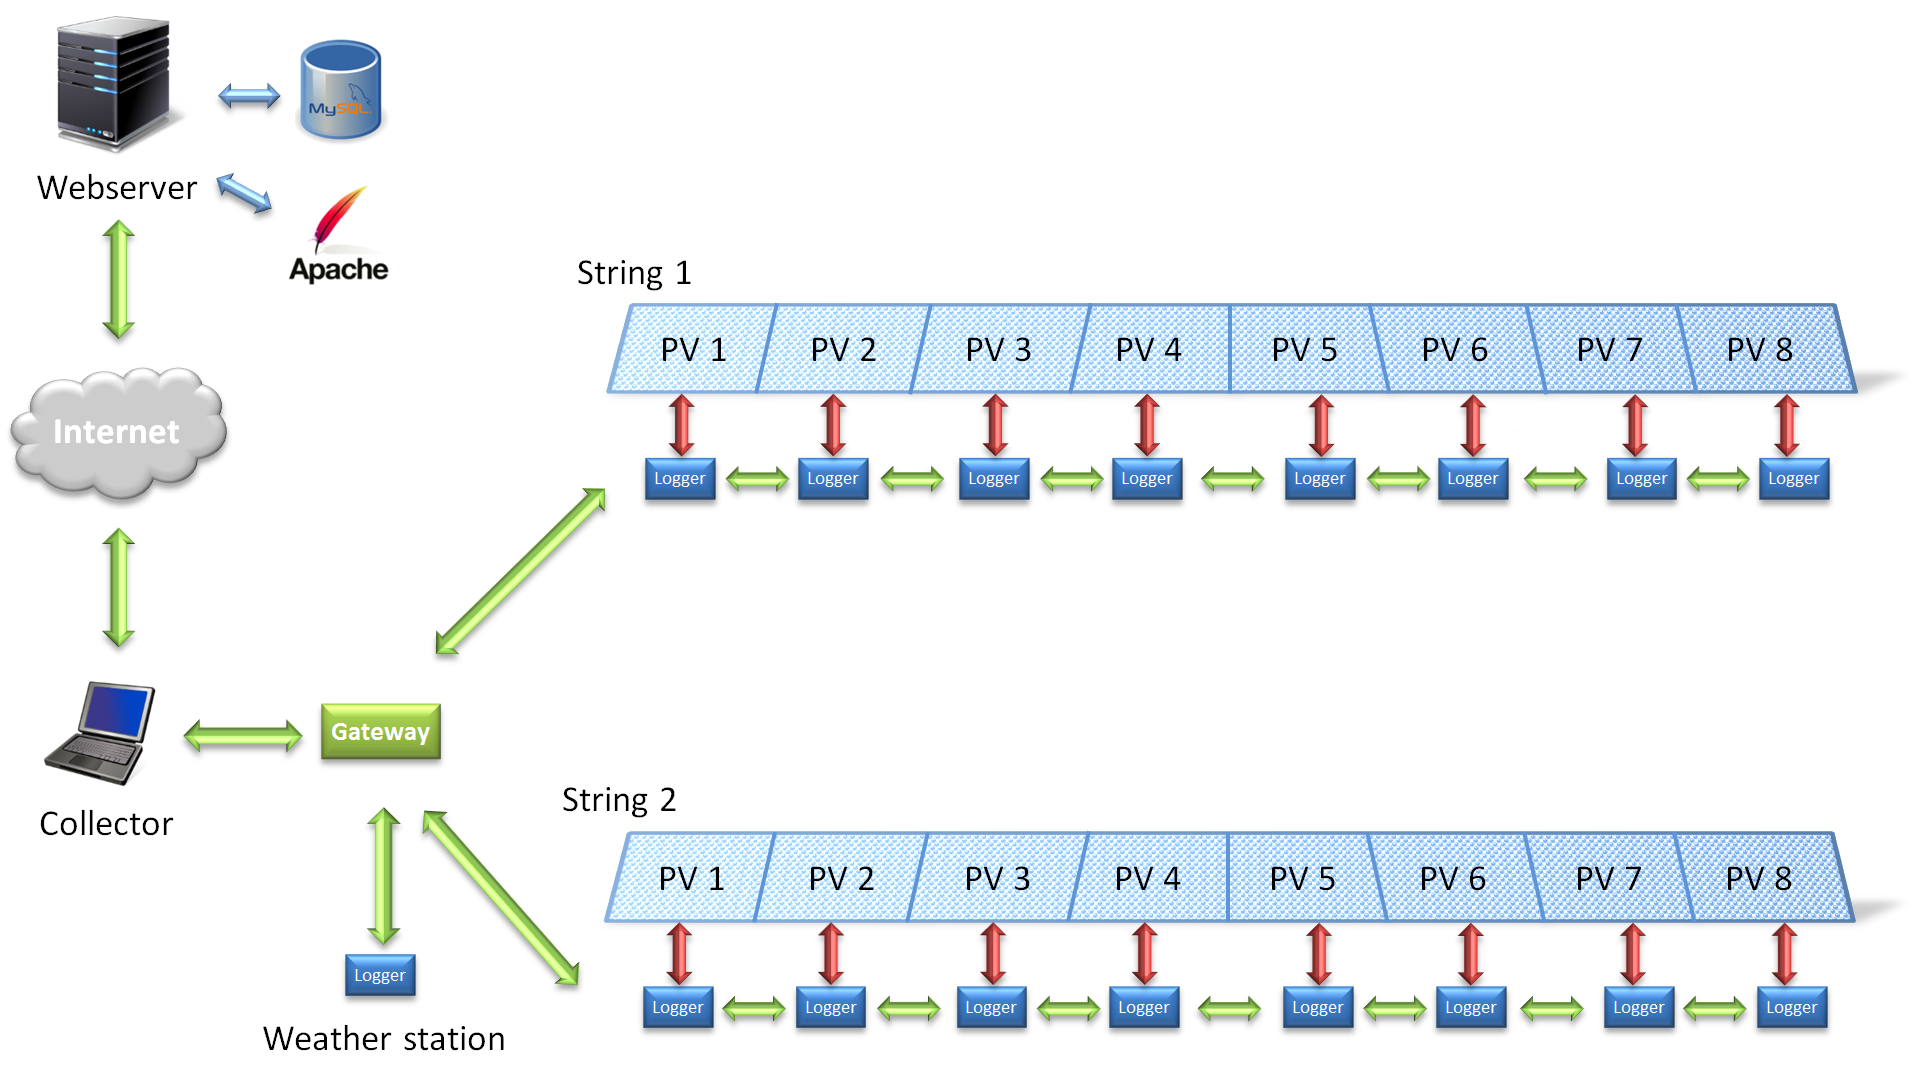
\includegraphics[width=0.80\textwidth]{../figures/large1.png}
	\caption{Beschriftungstext}
	\label{fig:large1}
\end{figure}

\subsection{Zwei Bilder nebeneinander oder untereinander}
%%%%%%%%%%%%%%%%%%%%%%%%%%%%%%%
\begin{figure*}[!htb]
	\centering
	\subfigure[Beschriftung Bild links]{
	  \label{fig:small1}
		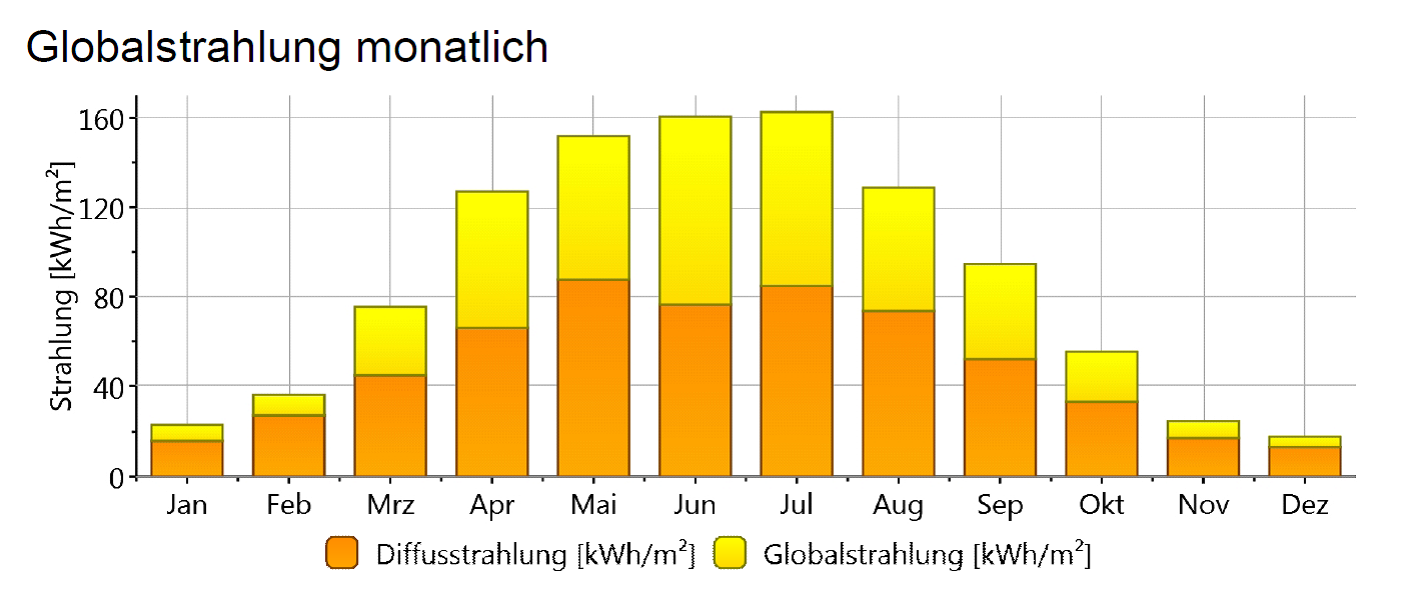
\includegraphics[angle=0,width=0.68\textwidth]{../figures/small1.png}}
	\subfigure[Beschriftung Bild rechts]{
	  \label{fig:small2}
		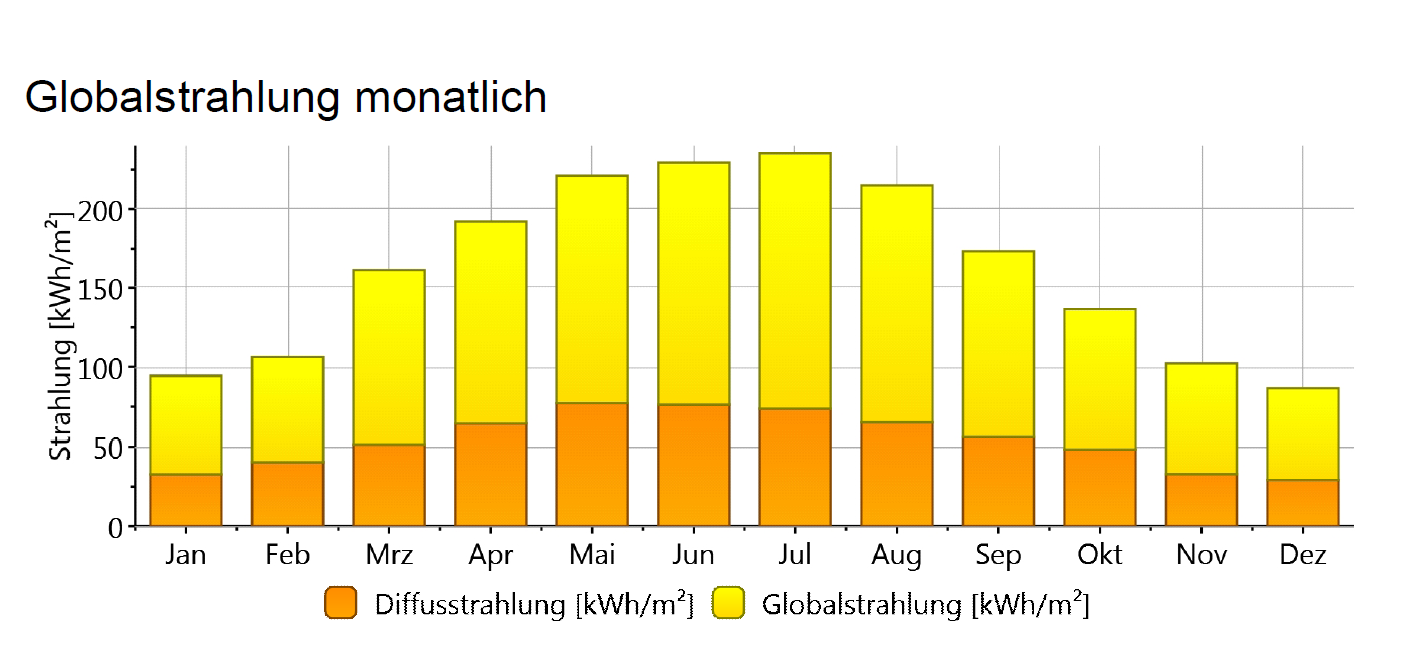
\includegraphics[angle=0,width=0.68\textwidth]{../figures/small2.png}}
 	\caption{Beschriftung beide Bilder} 
	\label{fig:beidebilder}
\end{figure*}
%%%%%%%%%%%%%%%%%%%%%%%%%%%%%%%


%% ==============================
\section{Tabellen}
%% ==============================
\begin{table}[htbp]
	\centering
		\begin{tabular}{|l|L{3.3 cm}|L{6.1 cm}|}
			\hline
			Firma								&			Produkte / L�sungen											&		WEB\\
			\hline
			Concentrix (Soitec)	&	Module mit Konzentratoren (Fresnel-Linsen)	&	http://www.soitec.com \\
			\hline
			Isofoton						&	Module mit Konzentratoren (Fresnel-Linsen)	&	http://www.isofoton.com \\
			\hline
			Semprius						& Module mit Konzentratoren (Fresnel-Linsen)	& http://www.semprius.com \\ 
			\hline
			\hline
			Azur Space					& Mehrfach Junction Zellenhersteller					& http://www.azurspace.com \\
			\hline
			Cyrium Technologies	& Mehrfach Junction Zellenhersteller					& \small{http://www.cyriumtechnologies.com} \\
			\hline
			Emcore							& Mehrfach Junction Zellenhersteller					& http://www.emcore.com \\
			\hline
		\end{tabular}
	\caption{Hersteller von CPV-Produkten}
	\label{tab:Hersteller}
\end{table}

\begin{table}[htb]
		\centering
		%\renewcommand{\arraystretch}{1.03}
		\caption{Single-hop Scenario - Traffic Pattern \label{t:traffic}}
			
		\begin{tabular}{l@{~}l@{\,\,}l@{\,\,}l} \hline \rule{-2pt}{12pt}
			Pattern& Parameter & Distribution & Range/Values  \rule{0pt}{12pt} \\ \hline \rule{-2pt}{12pt}  
      \textbf{Burst}      
      & Burst IAT         & uniform  & [9.9; 10.1] s\\ 
      & Packets per Burst & constant & 100\\
      & Packet IAT        & constant & 0.02 s\\
      & Packet Size       & constant & 1024 bit\\
      & \# Sources & -        & 2\\
			& Offset						& uniform  & [0; 1] s\\ 
      \hline      \hline\rule{-2pt}{12pt} 
      \textbf{Single}     & Packet IAT        & uniform  & [0.9; 1.1] s\\
      & Packet Size       & constant & 1024 bit\\
      & \# Sources & -        & [10;20;30;40;50;\\
      & & & 60;70;80;90;100]\\
			& Offset						& uniform  & [0; 1] s\\ 
      \hline
    \end{tabular}
\end{table}   % Beispiele
%% analyse.tex
%%

\chapter{Analyse}
\label{ch:Analyse}
%% ==============================
Bla fasel\ldots

%% ==============================
\section{Abschnitt 1}
%% ==============================
\label{ch:Analyse:sec:Abschnitt1}

Bla fasel\ldots

%% ==============================
\section{Abschnitt 2}
%% ==============================
\label{ch:Analyse:sec:Abschnitt2}
Bla fasel\ldots
\subsection{Unterabschnitt}
Bla fasel\ldots
\subsubsection{Unter-Unterabschnitt}

     % Analyse

%% ++++++++++++++++++++++++++++++++++++++++++
%% Anhang
%% ++++++++++++++++++++++++++++++++++++++++++

%\appendix
%\chapter{Material}
\label{ch:Material}
\enlargethispage{120cm}
\section{PMOD-Pinbelegung des IceZero-Boards}

Bei der Pin-Belegung wurde das selbe Schema wie beim GPIO-Modul des IcoSoc verwendet. Die Numerierung läuft dementsprechend von rechts nach links und für die einzelnen PMOD-Header ``zeilenweise'' von oben nach unten.

\begin{figure}[h]
	\centering
	\captionsetup{justification=centering,margin=2cm}
		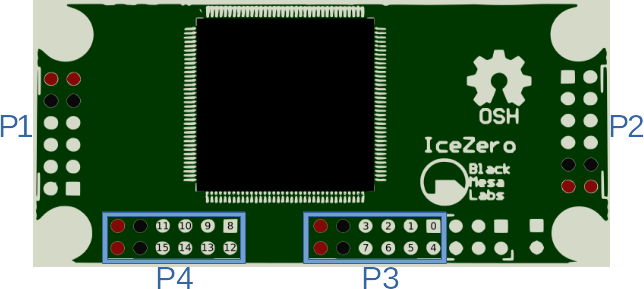
\includegraphics[width=0.80\textwidth]{../figures/ice40_pmod_pins_01.png}
		\caption[Pinbelegung der PMOD-Header des IceZero-Boards]{Pinbelegung der PMOD-Header des IceZero-Boards (Quelle: Eigene Abbildung)}
	\label{fig:ice40_pmod_pins}
\end{figure}

\begin{table}[h]
\centering
\resizebox{\columnwidth}{!}{%
\begin{tabular}{lllllllllllll}
\cline{1-6} \cline{8-13}
\multicolumn{1}{|l|}{\cellcolor[HTML]{DF2727}3.3V} & \multicolumn{1}{l|}{\cellcolor[HTML]{343434}{\color[HTML]{FFFFFF} GND}} & \multicolumn{1}{l|}{pin\_11} & \multicolumn{1}{l|}{pin\_10} & \multicolumn{1}{l|}{pin\_9}  & \multicolumn{1}{l|}{pin\_8}  & \multicolumn{1}{l|}{} & \multicolumn{1}{l|}{\cellcolor[HTML]{DF2727}3.3V} & \multicolumn{1}{l|}{\cellcolor[HTML]{343434}{\color[HTML]{FFFFFF} GND}} & \multicolumn{1}{l|}{pin\_3} & \multicolumn{1}{l|}{pin\_2} & \multicolumn{1}{l|}{pin\_1} & \multicolumn{1}{l|}{pin\_0} \\ \cline{1-6} \cline{8-13} 
\multicolumn{1}{|l|}{\cellcolor[HTML]{DF2727}3.3V} & \multicolumn{1}{l|}{\cellcolor[HTML]{343434}{\color[HTML]{FFFFFF} GND}} & \multicolumn{1}{l|}{pin\_15} & \multicolumn{1}{l|}{pin\_14} & \multicolumn{1}{l|}{pin\_13} & \multicolumn{1}{l|}{pin\_12} & \multicolumn{1}{l|}{} & \multicolumn{1}{l|}{\cellcolor[HTML]{DF2727}3.3V} & \multicolumn{1}{l|}{\cellcolor[HTML]{343434}{\color[HTML]{FFFFFF} GND}} & \multicolumn{1}{l|}{pin\_7} & \multicolumn{1}{l|}{pin\_6} & \multicolumn{1}{l|}{pin\_5} & \multicolumn{1}{l|}{pin\_4} \\ \cline{1-6} \cline{8-13} 
\multicolumn{6}{c}{PMOD - P4}                                                                                                                                                                                                                            &                       & \multicolumn{6}{c}{PMOD - P3}                                                                                                                                                                                                                      
\end{tabular}
}
\caption{Pinbelegung der PMOD-Header des Icezero-Boards}
\label{tbl:PMOD-Pins}
\end{table}


\clearpage
\begin{landscape}

\section{Pinverbindungen Raspberry Pi und FPGA-Shield}

\begin{table}[h]
\centering
\caption{Pinbelegung}
\label{tbl:Pinbelegung}
\begin{tabular}{|l|l|l|
>{\columncolor[HTML]{EFEFEF}}l |
>{\columncolor[HTML]{EFEFEF}}l |l|l|l|}
\hline
\cellcolor[HTML]{C0C0C0}ice40 & \cellcolor[HTML]{C0C0C0}WiringP & \cellcolor[HTML]{C0C0C0}Name                       & \multicolumn{2}{l|}{\cellcolor[HTML]{C0C0C0}Physical} & \cellcolor[HTML]{C0C0C0}Name                       & \cellcolor[HTML]{C0C0C0}WiringPi & \cellcolor[HTML]{C0C0C0}ice40 \\ \hline
                              &                                 & \cellcolor[HTML]{DF2727}3.3V                       & 1                         & 2                         & \cellcolor[HTML]{DF2727}5V                         &                                  &                               \\ \hline
                              & 8                               & SDA.1                                              & 3                         & 4                         & \cellcolor[HTML]{DF2727}5V                         &                                  &                               \\ \hline
                              & 9                               & SCL.1                                              & 5                         & 6                         & \cellcolor[HTML]{000000}{\color[HTML]{FFFFFF} GND} &                                  &                               \\ \hline
                              & 7                               & 1-Wire                                             & 7                         & 8                         & TxD                                                & 15                               &                               \\ \hline
                              &                                 & \cellcolor[HTML]{000000}{\color[HTML]{FFFFFF} GND} & 9                         & 10                        & RxD                                                & 16                               &                               \\ \hline
                              & 0                               & GPIO. 0                                            & 11                        & 12                        & GPIO.1                                             & 1                                &                               \\ \hline
                              & 2                               & GPIO. 2                                            & 13                        & 14                        & \cellcolor[HTML]{000000}{\color[HTML]{FFFFFF} GND} &                                  &                               \\ \hline
                              & 3                               & GPIO. 3                                            & 15                        & 16                        & GPIO. 4                                            & 4                                &                               \\ \hline
                              &                                 & \cellcolor[HTML]{DF2727}3.3V                       & 17                        & 18                        & GPIO. 5                                            & 5                                &                               \\ \hline
                              & 12                              & MOSI                                               & 19                        & 20                        & \cellcolor[HTML]{000000}{\color[HTML]{FFFFFF} GND} &                                  &                               \\ \hline
                              & 13                              & MISO                                               & 21                        & 22                        & GPIO. 6                                            & 6                                &                               \\ \hline
                              & 14                              & SCLK                                               & 23                        & 24                        & CE0                                                & 10                               &                               \\ \hline
                              &                                 & \cellcolor[HTML]{000000}{\color[HTML]{FFFFFF} GND} & 25                        & 26                        & CE1                                                & 11                               &                               \\ \hline
                              & 30                              & SDA.0                                              & 27                        & 28                        & SCL.0                                              & 31                               &                               \\ \hline
			      & 21                              & GPIO.21                                            & 29                        & 30                        & \cellcolor[HTML]{000000}{\color[HTML]{FFFFFF} GND} &                                &                               \\ \hline
                              & 22                              & GPIO.22                                            & 31                        & 32                        & GPIO.26                                            & 26                               &                               \\ \hline
                              & 23                              & GPIO.23                                            & 33                        & 34                        & \cellcolor[HTML]{000000}{\color[HTML]{FFFFFF} GND} &                                &                               \\ \hline
                              & 24                              & GPIO.24                                            & 35                        & 36                        & GPIO.27                                            & 27                               &                               \\ \hline
                              & 25                              & GPIO.25                                            & 37                        & 38                        & GPIO.28                                            & 28                               &                               \\ \hline
                              &                                 & \cellcolor[HTML]{000000}{\color[HTML]{FFFFFF} GND} & 39                        & 40                        & GPIO.29                                            & 29                               &                               \\ \hline
\end{tabular}
\end{table}
\end{landscape}

\clearpage

\section{CD}
Die beiliegende CD enthält den Inhalt des Github-Repositories 
\begin{lstlisting}[language=bash]
https://github.com/dm7h/fpga-event-recorder
\end{lstlisting}
zum Zeitpunkt der Abgabe.

Folgende Tabelle entält einen Überblick über die Inhalte des Repositories:
\begin{table}[h]
\centering

\begin{tabular}{|p{1cm}|p{3cm}|p{10cm}|}
\hline
\rowcolor[HTML]{C0C0C0} 
Verz. & Unterverzeichnis                & Inhaltsbeschreibung                                                                                                                                                                                                                                                                                                      \\ \hline
doc/        & ref/                            & iCE40 Manuals und relevante Hardwaredokumentation                                                                                                                                                                                                                                                                        \\ \hline
thesis/     &                                 & Finale Version der Bachelorarbeit als PDF                                                                                                                                                                                                                                                             \\ \hline
thesis/     & src/                            & Latex-Sourcen der Bachelorarbeit                                                                                                                                                                                                                                                              \\ \hline
src/        &                                 &                                                                                                                                                                                                                                                                                                                          \\ \hline
            & Logikanalysator/                & Dateien des Semesterprojekts ``Logikanalysator mit AVR Mega32U4 und Altera MAX CPLD''  inkl. Dateien der Bachelorarbeit von Andreas Müller (USB-TPLE)  
															     \\ \hline
            & icotools/                       & Portierung des icotools Projekts für das IceZero-Board. Original-Repository: https://github.com/cliffordwolf/icotools. Relevant sind hier vor allem die Unterverzeichnisse ``icosoc'' und ``icoprog'' 
\\ \hline
            & icozctl/                        & Fork des icoprog-Tools (icotools/icoporg) mit zusätzlichen Funktionen zur Steuerung des Event-Recorders                                                                                                                                                                                                                  \\ \hline
            & icozero/                        & Vom IcoSoc unabhängiges Beispiel-Projekt für das IceZero-Board mit leichten Modifikationen (nicht projekt-relevant)                                                                                                                                                                                                      \\ \hline
            & picosoc/                        & Portierung des PicoSoc-Projekts auf das IceZero-Board (nicht direkt projekt-relevant). PicoSoc ist eine minimale Variante des IcoSocs. Original-Repository: https://github.com/cliffordwolf/picorv32/tree/master/picosoc                                                    \\ \hline
            & sump2/                          & SUMP2 Variante für das IceZero-Board (nicht für die Icestorm-Toolchain)                                                                                                                                                                                                                                                  \\ \hline
            & sump2\_pipistrello\_ ftdi\_fifo/ & SUMP2 Vairante für das Pipistrello-Board bei dem der Versuch unternommen wurde den UART durch einen FTDI-Fifo zu ersetzen, um einen Höheren Datenduchsatz zu ermöglichen. Quelle: http://forum.gadgetfactory.net/topic/1748-open-bench-logic-sniffer-with-64mb-capture-buffer/ \\ \hline
            & demon-core-import/              & SUMP2 Weiterenwicklung für den Open Bench Logic Sniffer. Quelle: https://github.com/jhol/demon-core-import                                                                                                                                                                     \\ \hline
\end{tabular}
\caption{Überblick über den Inhalt des Git-Repositories}
\label{tbl:git_repo}
\end{table}

%\chapter{GPL}
\label{ch:GPL}
%% ==============================
Anhang B \ldots



\ifnotonesideelse{\cleardoublepage}{}

%% ++++++++++++++++++++++++++++++++++++++++++
%% Literatur
%% ++++++++++++++++++++++++++++++++++++++++++
\addcontentsline{toc}{chapter}{\bibname}
%  mit dem Befehl \nocite werden auch nicht zitierte Referenzen abgedruckt 
% (normalerweise nicht erwünscht)
% \nocite{*}
\bibliographystyle{rialpha}
%Einbinden Bibtexdatei - Direkt aus JabRef generiert
\bibliography{literatur}
%% ++++++++++++++++++++++++++++++++++++++++++
%% Index (optional)
%% ++++++++++++++++++++++++++++++++++++++++++
%\ifnotdraft{
%\addcontentsline{toc}{chapter}{Index}
%\printindex            % Index, Stichwortverzeichnis
%}
\end{document}
